\chapter{Resultados: What Weee Are Game}
\label{resultados}

Neste capítulo é detalhado aspectos presentes do jogo "What Weee Are" e os motivos da escolha. A história se desenrola em quatro cenários: Cozinha, Jardim, Metrô e Vulcão, descrição das personagens, explicação da escolha dos planos de fundo e o enredo do jogo estão presentes neste capítulo. Todos os detalhes de implementação, aplicabilidade e escolhas para o jogo, as explicações de mecânicas como o sistema de crafting e a discussão final.

\section{Enredo}
Em "What Weee Are", somos apresentados a Weee, o herói da história que enfrentará desafios e se fortalecerá para combater a Eco-InterCrim, a grande vilã da aventura. Weee tem como objetivo coletar os materiais descartados incorretamente ao longo de sua jornada e usá-los para limpar o planeta das mãos da Eco-InterCrim, organização criminosa responsável pela poluição do meio ambiente por meio do descarte inadequado de resíduos eletrônicos.

Acompanhando Weee em sua missão, está o Grilo Falante, um sábio guia que fornece informações sobre a situação e orienta o personagem jogável pelo mundo, explicando o que deve ser feito para progredir. O Grilo Falante aparece em diálogos ao longo do jogo e no início de cada cenário, fornecendo instruções e contexto para a jornada de Weee.

A aventura se inicia no cenário da Cozinha, onde o Grilo Falante revela os problemas causados pelo descarte inadequado de resíduos eletrônicos e apresenta a Eco-InterCrim como a possível responsável por essa situação. Weee deve enfrentar desafios como coletar itens e derrotar formigas vermelhas e verdes, culminando em um confronto com a Aranha Mecânica, o desafio final do cenário.

No cenário do Jardim, Weee recebe a informação de que pode adquirir uma nova habilidade, o pulo-duplo, para investigar possíveis contaminações. O Grilo Falante indica a necessidade de voltar à Cozinha para coletar mais itens e construir essa nova habilidade. Ao chegar no Jardim, Weee encontra fluidos poluentes, agravando a situação e indicando a gravidade dos crimes ecológicos cometidos pela Eco-InterCrim.

O próximo cenário é o Metrô, onde o Grilo Falante revela que a Eco-InterCrim está usando a malha ferroviária para disseminar seus crimes ambientais por meio do plano chamado Toxicity. Weee deve avançar até o vulcão, enfrentando desafios e coletando itens, como o potencializador de pulos, para aprimorar suas habilidades e combater a organização.

O último desafio ocorre no cenário do Vulcão, onde a base da Eco-InterCrim está localizada. Weee enfrenta riscos, como a presença de lava, enquanto busca acabar com os planos da organização criminosa. Ao finalizar essa etapa, Weee é parabenizado por seu feito heroico e é informado de que agora é necessário lidar com os danos causados pela Eco-InterCrim.

O jogo termina com a missão de Weee retornar à Cozinha para coletar mais itens e auxiliar na reconstrução do planeta. Embora haja o risco de que a Eco-InterCrim volte a atacar, Weee está agora ciente da identidade dos responsáveis e está determinado a impedir que os crimes ecológicos ocorram novamente, protegendo o meio ambiente.

%\section{What Weee Are: The Game}
\section{Personagens}
A escolha de todos os personagens e inimigos é resultado de uma colaboração criativa liderada por Alessio, que já vinha desenvolvendo criaturas feitas exclusivamente a partir de materiais eletrônicos reciclados. Sua participação artística foi fundamental ao fornecer as ilustrações que compõem o jogo. A inclusão de personagens construídos a partir de materiais reciclados serve como uma poderosa forma de reforçar a mensagem central do jogo em relação ao tema ambiental.

What Weee Are possui dois personagens principais. Weee, a formiga e o Grilo Falante. Weee é nosso personagem controlável, onde iremos andar e explorar pelos quatro cenários que encontramos no jogo, Weee será capaz de coletar itens, destruir itens complexos, montar itens, desmontar itens, adquirir novas habilidades, derrotar inimigos e assim progredir cada vez mais pelo mundo.

Weee é o herói da história, que irá enfrentar os desafios, se fortalecer e por fim enfrentar o grande inimigo da aventura, a Eco-InterCrim. Weee coletará os materiais descartados incorretamente e propositalmente ao longo da jornada, usará tudo que tiver disponível para alcançar o seu objetivo de limpar o planeta das mãos da Eco-InterCrim

\begin{figure}[h]
    \centering
    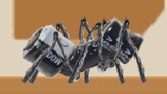
\includegraphics[width=150px]{figuras/weee.png}
    \caption{Weee - o personagem jogável}
    \label{fig_weee}
\end{figure}
\par
O Grilo Falante é o guia de Weee, é quem irá contar o que está acontecendo e direcionará o personagem jogável pelo mundo e o que deverá fazer para progredir. Haverão diálogos durante o jogo e no início dos cenários onde o Grilo irá aparecer para interagir.
\begin{figure}[h]
    \centering
    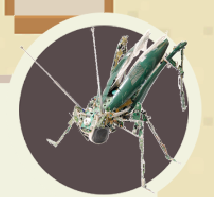
\includegraphics[width=150px]{figuras/grilo.png}
    \caption{Grilo Falante - o guia}
    \label{fig_grilo}
\end{figure}

\section{Cenários}
Esta seção apresentará quatro cenários distintos do jogo "What Weee Are": Cozinha, Jardim, Metrô e Vulcão. A escolha desses planos de fundo tem como objetivo demonstrar aos jogadores as consequências resultantes do descarte inadequado de materiais eletrônicos. Cada cenário representa uma situação única em que problemas relacionados ao descarte incorreto podem afetar tanto o ambiente doméstico quanto a sociedade em geral. Através dessas experiências virtuais, os jogadores serão confrontados com desafios que vão desde questões pessoais, como problemas dentro de casa, até problemas sociais, como a tentativa de contaminação do solo. O objetivo é fornecer uma perspectiva abrangente sobre os impactos negativos que a falta de gerenciamento adequado dos resíduos eletrônicos pode causar em diferentes contextos, incentivando assim a conscientização e a adoção de práticas sustentáveis.

\subsection{Fase 1 - A Cozinha}
Descrição: Nesta fase do jogo, somos apresentados ao que iremos enfrentar e algumas noções básicas do jogo. Aqui o Grilo Falante diz sobre como faremos a movimentação e como progredir durante a primeira fase. Irá dizer o que está acontecendo sobre o desperdício de materiais eletrônicos e quem possivelmente está causando isso. Devido ao abandono dos materiais em locais inapropriados, começaram a vazar substâncias tóxicas para o meio ambiente, e introduzirá a organização Eco-InterCrim como possíveis responsáveis pelo desastre.
Aparecerão alguns itens a serem coletados e algumas formigas vermelhas e verdes para enfrentar, além de uma Aranha Mecânica no final que será o maior desafio presente.

Sua escolha vêm como forma de apresentar o problema do descare incorreto dos materiais eletrônicos, mostrando que o problema também pode afetar em nossos ambientes privados. Além também de ser um estágio introdutório, pois o jogo segue uma linha de progressão entre os cenários.
\begin{figure}[h]
    \centering
    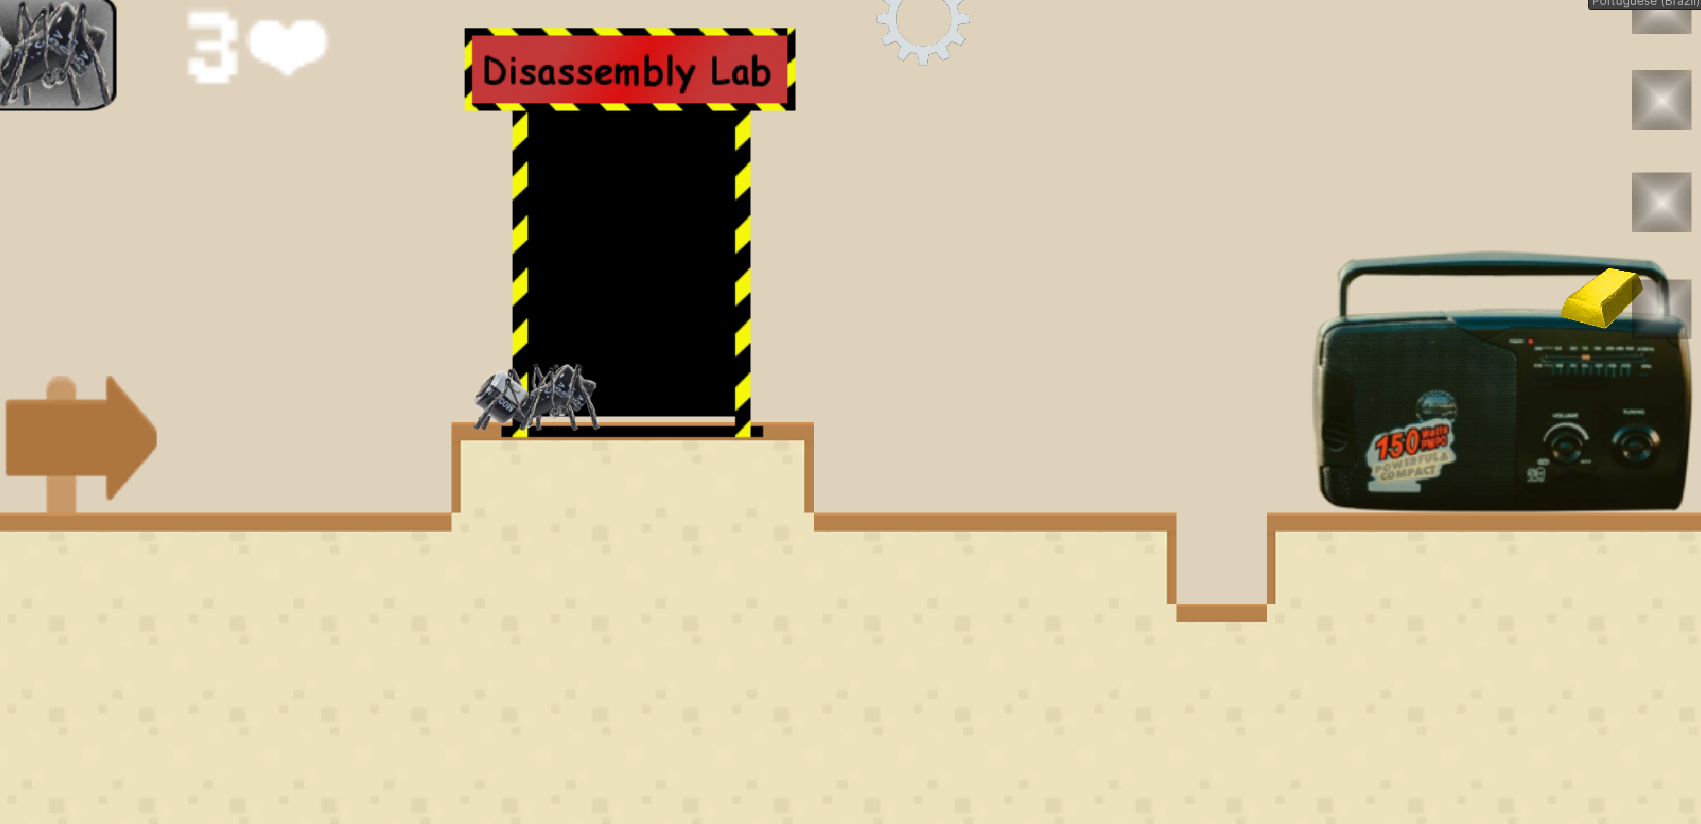
\includegraphics[width=300px]{figuras/cozinha.png}
    \caption{Fase 1 - A cozinha}
    \label{fig_cozinha}
\end{figure}

Música utilizada "Cookie Island" \cite{CookieIsland}

\subsection{Fase 2 - Jardim}

Descrição: Nesta etapa, o Grilo Falante nos dirá que é possível conseguir uma nova habilidade, o pulo-duplo e com isso investigar possíveis contaminações no Jardim. É informado da possibilidade de voltar à cozinha para coletar mais itens para ajudar a construir a nova habilidade.

A escolha do jardim vem como uma proposta de transição o lado de dentro (casa) e o mundo exterior, um estágio para servir como uma transicão entre a cozinha e o metrô.
\begin{figure}[h]
    \centering
    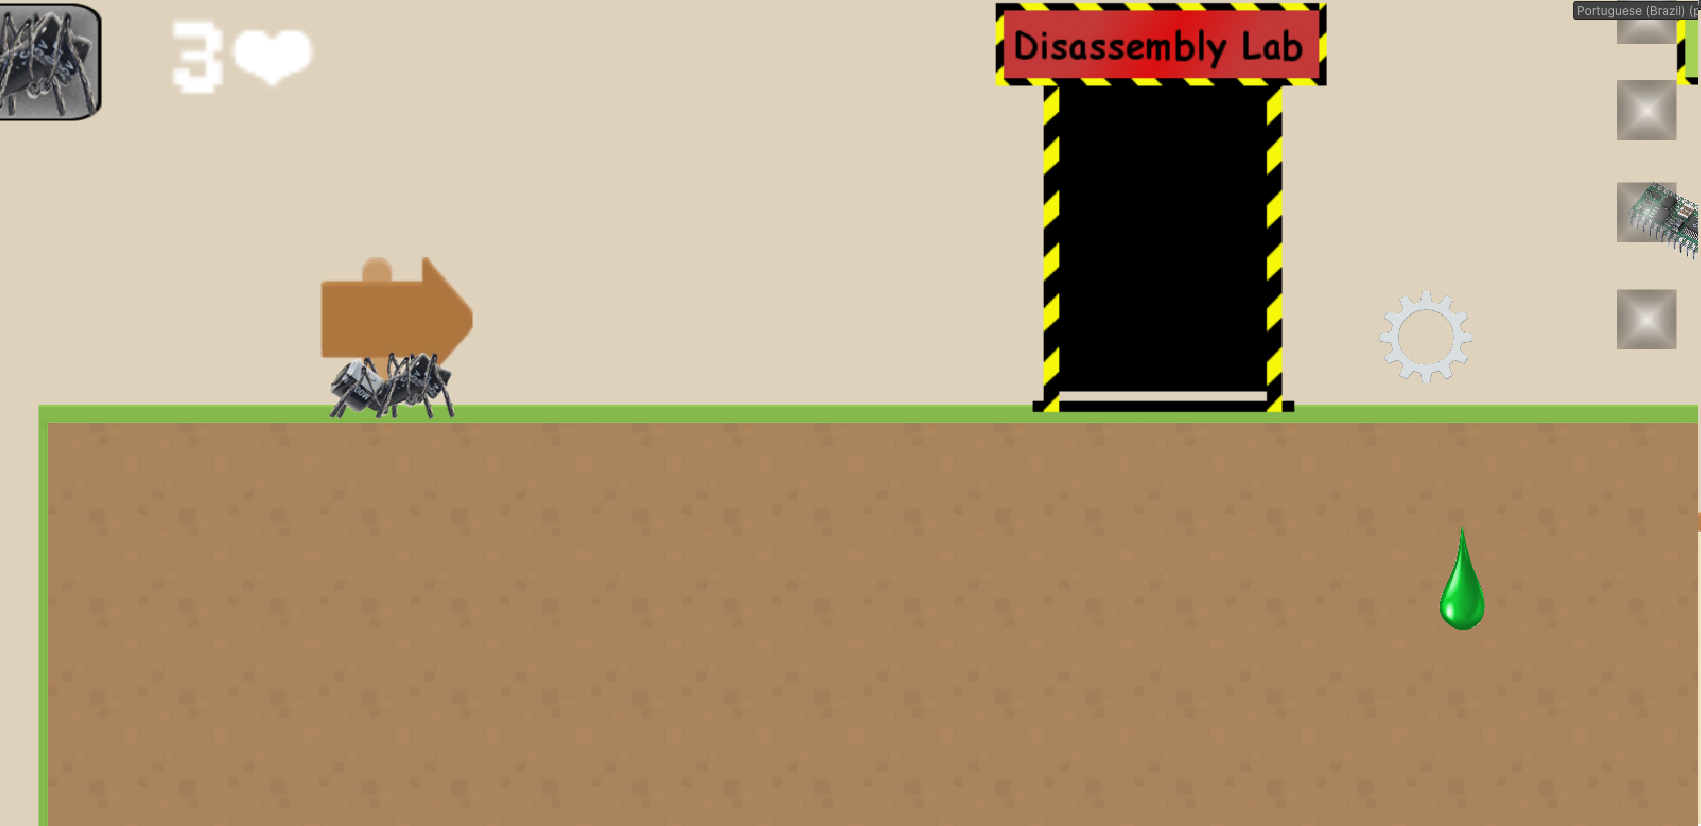
\includegraphics[width=300px]{figuras/jardim.png}
    \caption{Fase 2 - O jardim}
    \label{fig_jardim}
\end{figure}

Música utilizada "Candy Valley" \cite{CandyValley}

\subsection{Fase 3 - Metrô}
Descrição: Chegando no metrô, o Grilo Falante informa que a Eco-InterCrim está utilizando a malha ferroviária para disseminar seus crimes ambientais com seu plano Toxicity, tomando inicialmente o controle do subsolo e contaminando-o com, aumentando o risco de contaminação dos lençóis freáticos, os objetivos da organização é contaminar o planeta com lixo eletrônico, para que a população fique doente e dependente de seus produtos e serviços, que serão oferecidos como solução para os problemas causados por eles mesmos, a missão passa a ser de coletar o máximo de resíduos(itens) possíveis. 

Este cenário vem como plano de fundo para apresentar problemas sérios que o descarte inadequado pode causar à sociedade, como exemplificado no jogo o problema da contaminação do solo.
\begin{figure}[h]
    \centering
    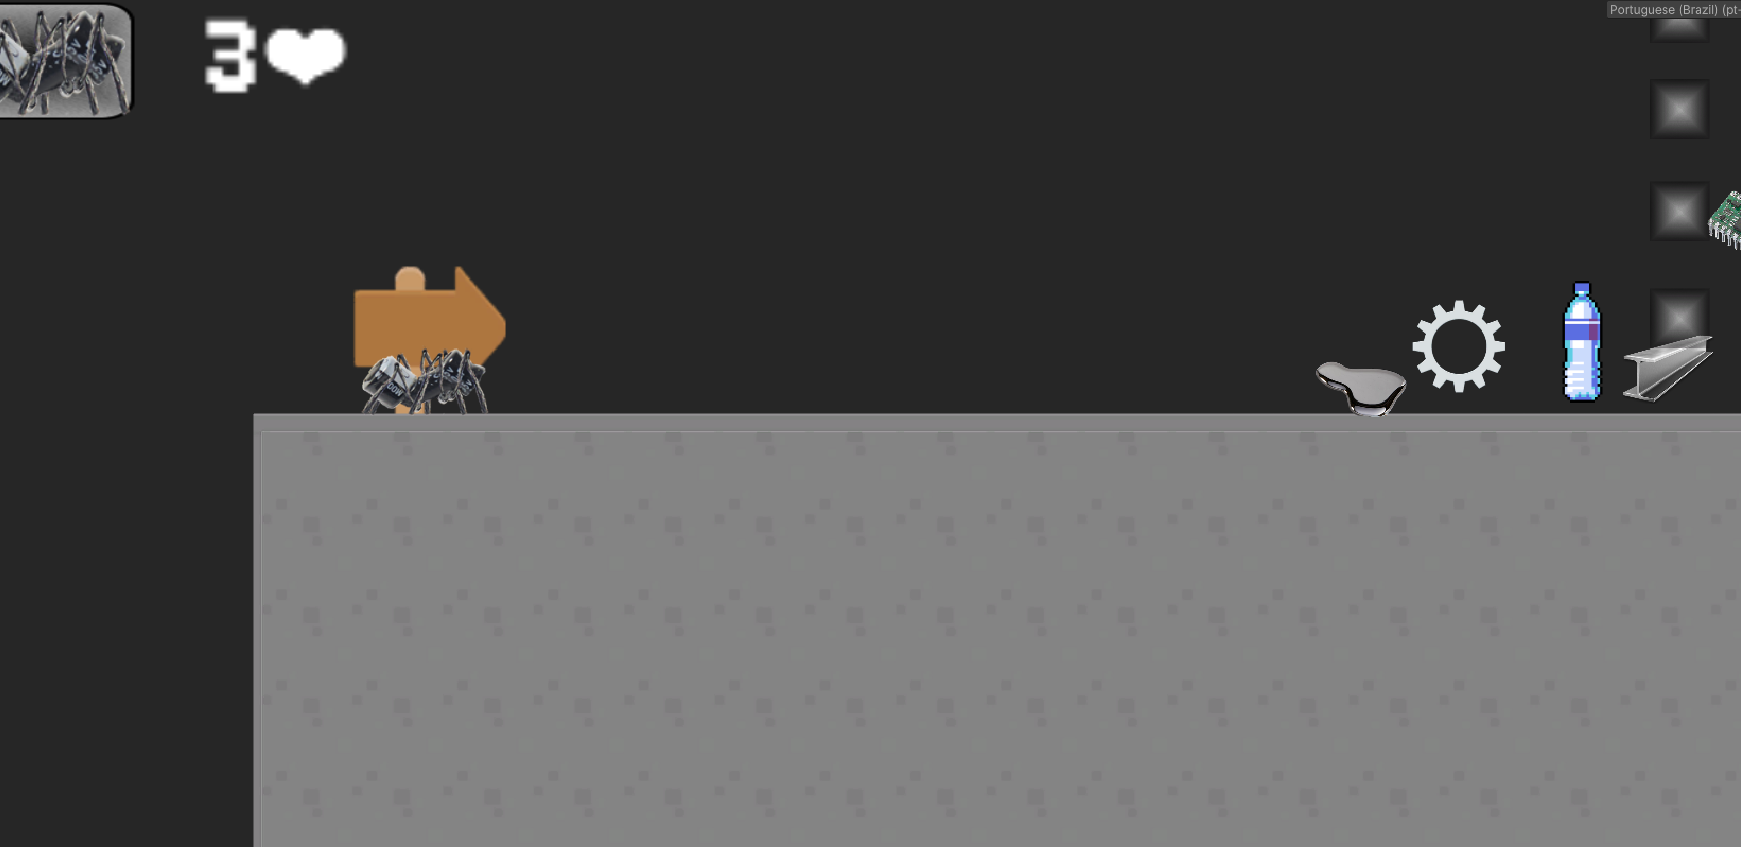
\includegraphics[width=300px]{figuras/metro.png}
    \caption{Fase 3 - O Metrô}
    \label{fig_metro}
\end{figure}

Música utilizada "Cyber Soldier" \cite{CyberSoldier}
\pagebreak

\subsection{Fase 4 - Vulcão}
O último desafio é o vulcão, aqui que está a base da Eco-InterCrim, onde finalmente será possível impedir que as investidas contra o meio ambiente tenham sucesso. Ao finalizar, Weee é parabenizada pelo seu feito heroico e que agora devemos cuidar dos danos causados pela organização criminosa.

Por fim este cenário foi escolhido como uma maneira de apresentar algo grandioso, um cenário de maior impacto visual e que passe a sensação de que algo importante está acontecendo no momento, justamente por ser o último estágio.
\begin{figure}[hbt!]
    \centering
    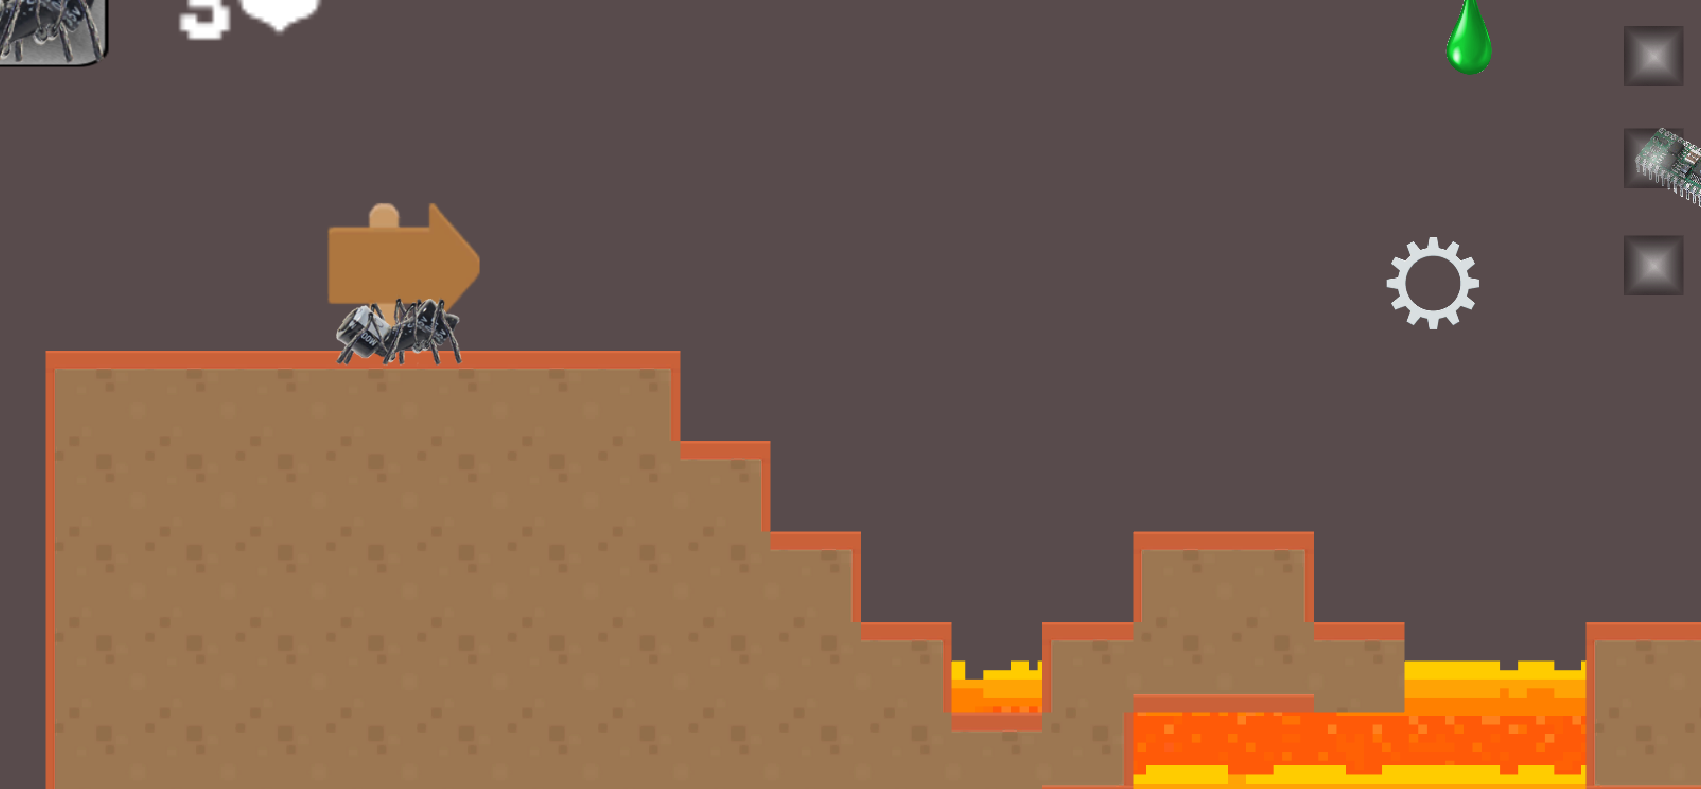
\includegraphics[width=300px]{figuras/vulcao.png}
    \caption{Fase 4 - O Vulcão}
    \label{fig_vulcao}
\end{figure}

Música utilizada "Final Act" \cite{FinalAct}

\section{Itens}
A seguir estão todos os itens presentes no jogo e a receita para construí-los (se possível), a existência também de alguns itens do jogo que podem aplicar algum efeito em Weee (e.g A bateria). As escolhas dos itens são justamente por serem subprodutos e resíduos eletrônicos e assim manter o tema central abordado no jogo e justificarem o uso do Sistema de \textit{Crafting} \ref{craft}
\label{list:itens}
\begin{itemize}
    \item Placa - Pode ser desmontado em ouro e ferro
    \item Cobre
    \item Engrenagem - Pode ser desmontado em prata
    \item Ouro
    \item Bateria - Dá vida à Weee, pode ser criado a partir de Aço e Mercúrio
    \item Ferro
    \item Mercúrio
    \item Plástico
    \item Prata
    \item Aço - Pode ser produzido a partir de 6 unidades de Ferro
\end{itemize}

\pagebreak
\section{Melhorias}
As melhorias a seguir, propõem a possibilidade da reciclagem dos materiais coletados durante as partidas pelos jogadores. Estas melhorias foram escolhidas como forma de trazer a sensação de progresso aos jogadores, confeccionadas por meio da reciclagem dos materiais coletados durante as fases do game.
\begin{itemize}
    \item Ganho de velocidade - Aumenta a velocidade por tempo determinado - Pode ser criado a partir de 14 únidades de placa e 10 unidades de engrenagem;
    \begin{figure}[hbt!]
        \centering
        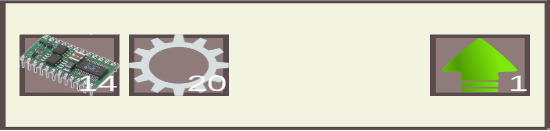
\includegraphics[width=300px]{figuras/receita_double_speed.png}
        \caption{Ganho de velocidade}
        \label{fig_receita_double_speed}
    \end{figure}
    
    \item Bateria - Dá vida à Weee - Pode ser criado a partir de Aço e Mercúrio;
    \begin{figure}[hbt!]
        \centering
        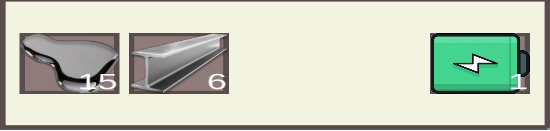
\includegraphics[width=300px]{figuras/receita_vida.png}
        \caption{Bateria}
        \label{fig_receita_vida}
    \end{figure}
    
    \item Pulo Duplo - Permite Weee realizar dois pulos subsequentes - Pode ser criado a partir de 12 unidades de placa, 11 unidades de engrenagem e 7 unidades de ferro;
    \begin{figure}[hbt!]
        \centering
        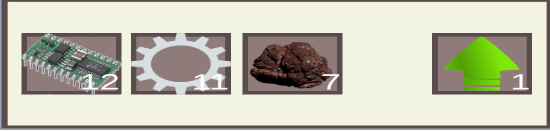
\includegraphics[width=300px]{figuras/receita_double_jump.png}
        \caption{Pulo Duplo}
        \label{fig_receita_double_jump}
    \end{figure}
    
    \item Aumento de Poder - Da a Weee a 4 vezes sua força atual, ideal para derrotar inímigos com um único golpe - Pode ser criado a partir de 14 unidades de mercúrio;
    \begin{figure}[hbt!]
        \centering
        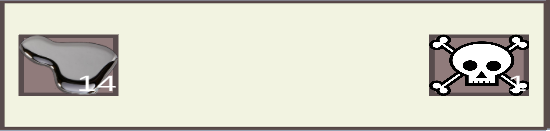
\includegraphics[width=300px]{figuras/receita.png}
        \caption{Aumento de Poder}
        \label{fig_receita_double_damage}
    \end{figure}
    
    \item Aumento de força de pulo - Da a Weee a capacidade de pular mais alto a cada pulo - Pode ser criado a partir de 12 unidades de engrenagem e 14 unidades de plástico.
    \begin{figure}[hbt!]
        \centering
        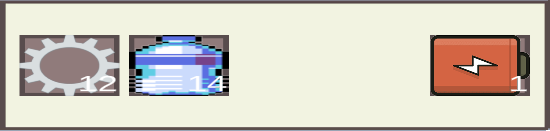
\includegraphics[width=300px]{figuras/receita_jump_force.png}
        \caption{Aumento de força de pul}
        \label{fig_receita_jump_force}
    \end{figure}
\end{itemize}

\section{Inimigos}
Os inimigos estão presentes para adicionar uma certa dificuldade no jogo e deixar a experiência mais divertida.
\begin{description}
    \item[Formigas Vermelhas] Apenas patrulham uma região. Criação artística do Alessio, a escolha deste inimigo vem de manter a estética de personagens insetos eletrônicos. 
    \begin{figure}[h]
        \centering
        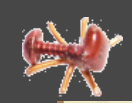
\includegraphics[width=100px]{figuras/redant.png}
        \caption{A Formiga Vermelha}
        \label{fig_redant}
    \end{figure}

    \item[Formigas Verdes] Patrulham uma região e podem pular. Criação artística do Alessio, a escolha deste inimigo vem de manter a estética de personagens insetos eletrônicos. Além de acrescentar uma dificuldade um pouco mais do que as formigas vermelhas.
    \begin{figure}[h]
        \centering
        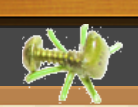
\includegraphics[width=100px]{figuras/greenant.png}
        \caption{A Formiga Verde}
        \label{fig_greenant}
    \end{figure}
    
    \item[Aranhas mecânicas] Possuem alta velocidade e podem pular. Criação artística do Alessio, a escolha deste inimigo vem de manter a estética de personagens insetos eletrônicos. Acrescentam uma dificuldade maior ainda do que das formigas verdes.
    \begin{figure}[h]
        \centering
        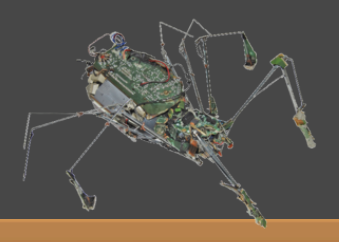
\includegraphics[width=100px]{figuras/spider.png}
        \caption{A Aranha Mecânica}
        \label{fig_spider}
    \end{figure}
\end{description}

\pagebreak
\section{Sistema de Crafting}
\label{craft}
A mecânica de \textit{"crafting"} é um conceito amplamente utilizado no design de jogos eletrônicos, que envolve a criação e destruição de elementos dentro do jogo, proporcionando uma experiência interativa aos usuários e estimulando sua criatividade. A criação e destruição são ações frequentemente presentes nesses jogos, fundamentais para essa mecânica.

Os sistemas de criação presentes nos jogos eletrônicos oferecem uma poderosa ferramenta para a criação de narrativas interativas, envolvendo os jogadores e permitindo a exploração de temas complexos. Para exemplificar esse argumento, o autor concentra-se no jogo de simulação urbana SimCity e em seu sistema de criação, que possibilita aos jogadores projetar e gerenciar cidades. De acordo com \cite{craftingGames}, o uso estratégico desse sistema de criação permite a criação de histórias complexas e interativas, que não apenas proporcionam uma experiência de jogo satisfatória, mas também exploram questões importantes, como o meio ambiente, a justiça social e as políticas públicas.

O sistema de "crafting" incorpora o conceito de reciclagem, permitindo que os jogadores utilizem materiais encontrados durante o jogo. Por meio desse sistema, é possível criar melhorias para o personagem, tornando-o mais forte, além de criar novos itens colecionáveis para a aventura. Dessa forma, esse sistema atribui importância à tarefa de coletar os itens necessários. \ref{list:itens}.

\subsection{Laboratório de desmontagem}
Aplicado os conceitos de Crafting voltados para desmontar itens complexos em itens primitivos, para assim criarmos outras opções de crafting
\begin{figure}[h]
    \centering
    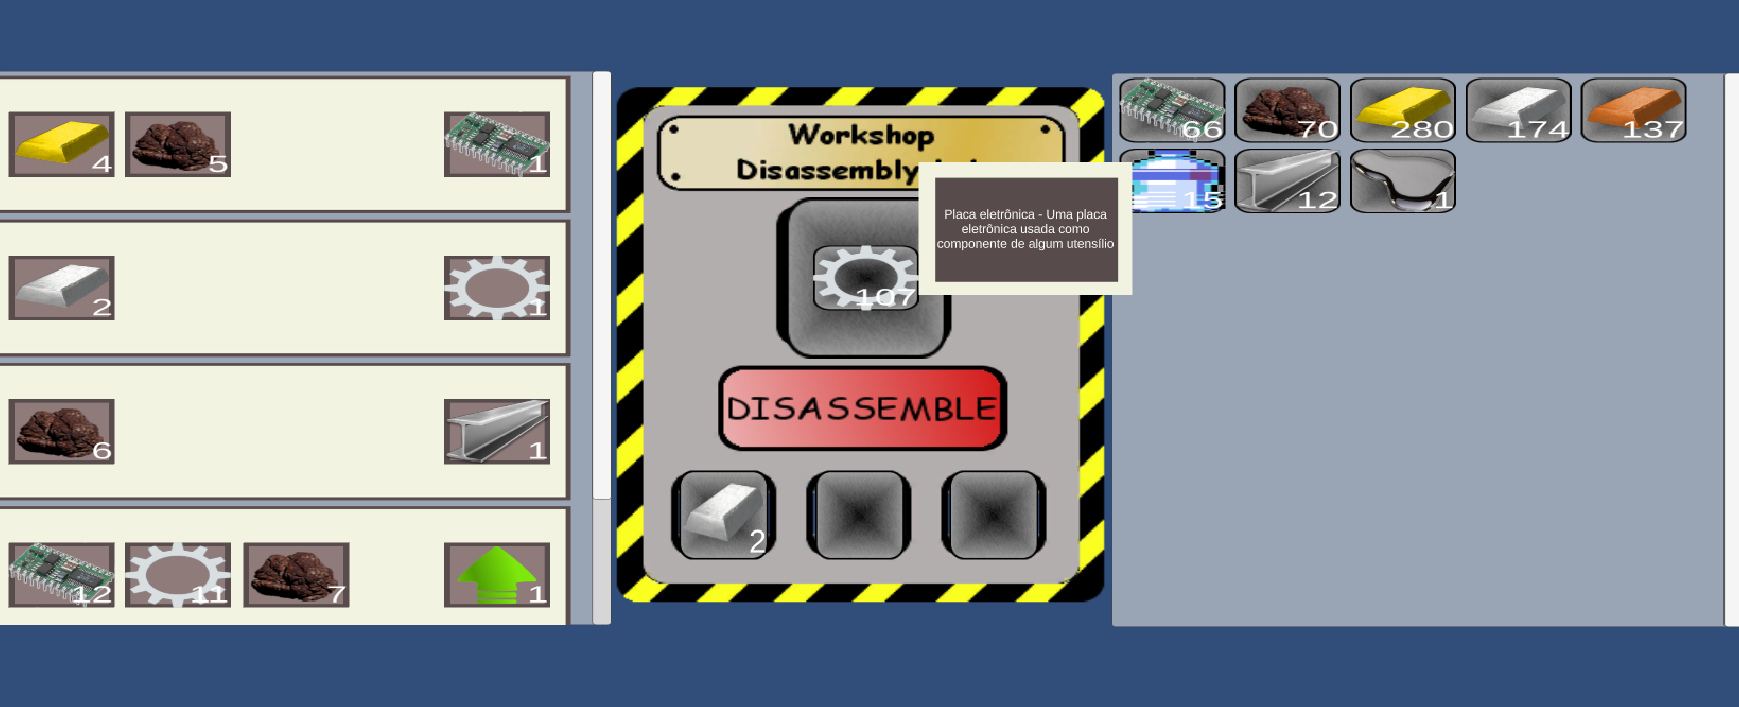
\includegraphics[width=500px]{figuras/disassembly.png}
    \caption{Laboratório de desmontagem - Desmontando um item}
    \label{fig_disassembler}
\end{figure}

\subsection{Laboratório de montagem}
Aplicado os conceitos de Crafting voltados para montar itens complexos ou novas habilidades para o jogador. A partir de receitas (que aponta quais itens são necessários para efetuar a criação), se o jogador oferecer os itens nas as quantidades necessárias, acontece com sucesso a operação.
\begin{figure}[h]
    \centering
    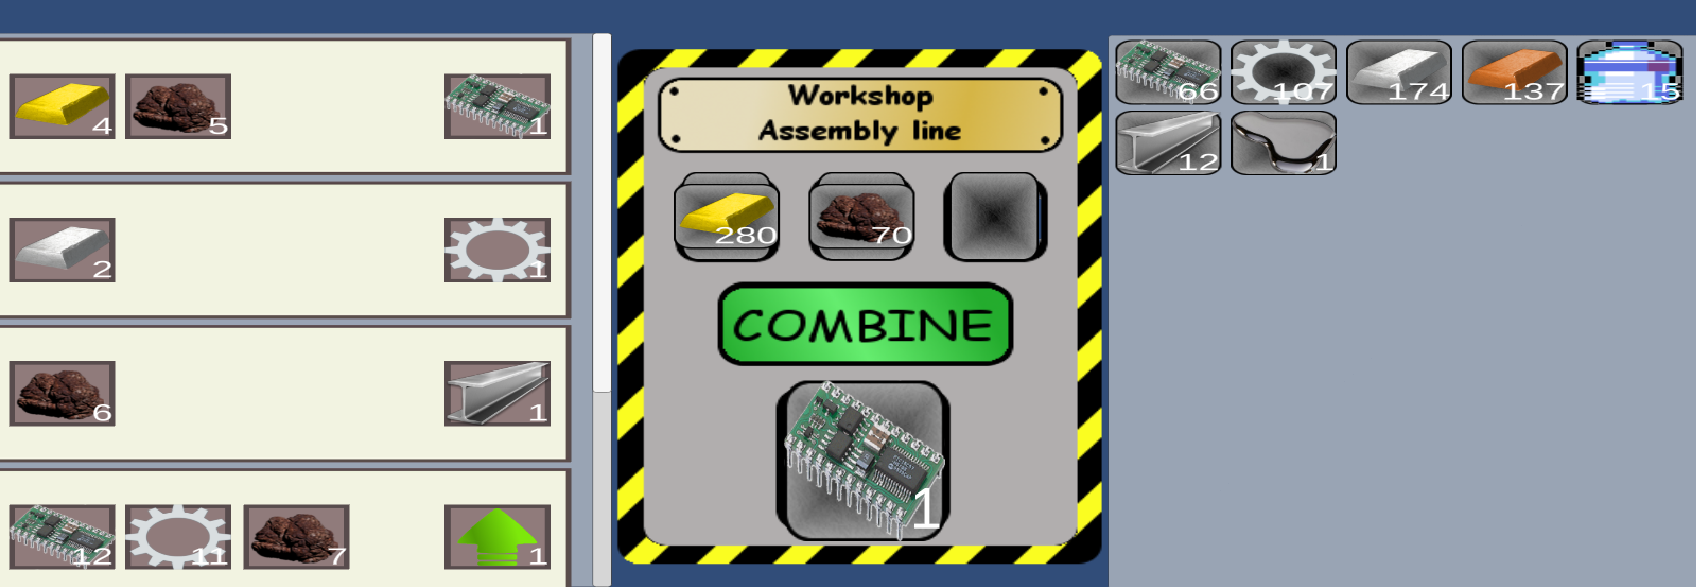
\includegraphics[width=500px]{figuras/assembly.png}
    \caption{Laboratório de montagem}
    \label{fig_assembler}
\end{figure}

\section{Discussão}
%Amarrar os conceitos de IHC com o desenvolvimento do jogo: como as personas foram usadas no desenvolvimento, cenários, análise de tarefas.
A crescente preocupação com questões ambientais é cada vez mais evidente na sociedade contemporânea e desempenha um papel crucial na busca por um futuro sustentável. O jogo em questão aborda especificamente a temática da preservação do meio ambiente, apresentando a organização criminosa Eco-InterCrim como responsável por desastres ambientais decorrentes do descarte inadequado de materiais. Essa abordagem tem o potencial de despertar o interesse dos jogadores e conscientizá-los sobre a importância da destinação correta de resíduos e ações voltadas para a redução do impacto humano no meio ambiente.

Além disso, o jogo transmite uma mensagem positiva, enfatizando que cada pessoa tem o poder de fazer a diferença ao agir em prol da proteção ambiental. O personagem Weee, por exemplo, assume o papel de herói ao frustrar os planos da organização criminosa. Adicionalmente, a mecânica de coleta de itens no jogo pode ser interpretada como uma forma de incentivar a reciclagem e a reutilização de materiais.

Com base nas personas definidas na (Tabela \ref{table:personasTable}), o desenvolvimento do jogo sugere ao jogador, por meio de dicas, a possibilidade de descobrir e aprender detalhes sobre o jogo. Um dos objetivos finais estabelecidos pela Análise Hierárquica de Tarefas (ver imagem \ref{fig_analise_hierarquica_b}) é justamente superar obstáculos, e uma maneira de introduzir dificuldades nesse objetivo é trazer a necessidade das personas de adquirir aprimoramentos para o personagem, outro objetivo final identificado na AHT (ver imagem \ref{fig_analise_hierarquica_c}). Para alcançar esses aprimoramentos, é necessário coletar os itens disponíveis em cada fase do jogo e derrotar os inimigos, que também são objetivos finais. O equilíbrio entre esses objetivos, aliado à proposta de aprendizado do jogo, visa proporcionar desafios para as personas e uma sensação de progresso a cada nova evolução alcançada (ver \ref{cenarios}), juntamente com a possibilidade de repetir as fases para acumular mais itens.

Embora o jogo não tenha a intenção de fornecer soluções concretas para os problemas ambientais, ele pode ser uma ferramenta eficaz para estimular a reflexão sobre a importância da preservação do meio ambiente e a responsabilidade individual em relação a esse tema. Educadores e professores podem utilizar o jogo como recurso em atividades de conscientização e educação ambiental, proporcionando uma abordagem lúdica para tratar de um assunto tão relevante.

Sob a óptica de IHC, What Weee Are se propõe a trazer os seguintes conceitos:

\begin{itemize}
    \item Usabilidade: O jogo deve ser fácil e intuitivo de jogar, com controles simples e fáceis de entender para que o jogador possa se concentrar na jogabilidade e na história do jogo.

    \item Feedback: O jogo deve fornecer feedback ao jogador sobre suas ações. Por exemplo, quando Weee coleta um item ou derrota um inimigo, o jogador deve receber uma notificação ou som para indicar que o objetivo foi alcançado.

    \item Design centrado no usuário: O jogo deve ser projetado pensando nas necessidades e preferências do usuário. Por exemplo, a interface deve ser clara e legível, com tamanho de fonte adequado e cores que não prejudiquem a visibilidade.

    \item Acessibilidade: O jogo deve ser acessível a um público amplo, incluindo pessoas com deficiência visual ou auditiva. Por exemplo, o jogo poderia ter opções de legendas ou opções de áudio para que os jogadores possam escolher a melhor forma de jogar.

    \item Consistência: O jogo deve ser consistente em toda a experiência do usuário, incluindo os controles, a aparência visual e a jogabilidade. Isso ajuda a garantir que o jogador não fique confuso ou frustrado enquanto joga.

    \item Personalização: O jogo poderia incluir opções de personalização, permitindo que os jogadores escolham sua própria aparência para o personagem ou o tipo de som que preferem ouvir.
\end{itemize}

Esses são apenas alguns exemplos de conceitos de Interação Humano-Computador que poderiam ser aplicados ao jogo "What Weee Are".
Inicialmente junto da persona João Pedro, o professor, foi utilizados seus conhecimentos acerca dos problemas causados pelo desperdício de materiais eletrônicos e como poderíamos aborda-los dentro do jogo. Contribuiu com a concepção do Sistema de Crafting (\ref{craft}), como mecânica que iria abordar como é possível reciclar e reatribuir uso a objetos, que antes seriam vistos como lixo, a se tornarem úteis novamente. As personas que iriam jogar o jogo, Natália e Leonardo, foram importante em como elaborar as fases e a dificuldade do jogo a ponto que, alunos de idade de 5 a 12 anos conseguissem prosseguir sem dificuldade, com uma linguagem simples que fosse capaz de apresentar o roteiro sem dificuldade de interpretação. Que fosse desafiador à alunos como Leonardo, que possuem facilidade em mecânicas de jogos, reaproveitando a comunicação simples. 
\par
O jogo foi desenvolvido em paralelo com a análise de tarefas, pois o jogo sofreu de influência de conceitos comumente apresentados em jogos muito conhecidos, plataforma 2D. Como
\begin{itemize}
    \item Super Mario World - Inspirou em como fazer uso de plataformas e dificuldade
    \item Donkey Kong Country - Inspirou em narrativa
    \item Megaman - Inspirou em conceitos de evolução de habilidades do personagem
    \item Minecraft - Inspirou no Sistema de Crafting
\end{itemize}

A partir destes conceitos distintos, a análise de tarefas junta-os em uma experiência com que seja possível fazer uso de forma contínua e fluida enquanto as personas jogam. O Professor João Pedro voltou a participar do processo de desenvolvimento, a fim de ajudar na escolha de quais itens seriam possível construir a partir do sistema de crafting, e quais upgrades estariam presentes em What Weee Are a partir da reciclagem dos materiais. 


